\documentclass{article}% use option titlepage to get the title on a page of its own.

\title{Tutorial k-Nearest Neighbours Regression}
\date{2020\\ August}
\author{Marcos del Cueto}

\usepackage{amsmath}
\usepackage{mathtools}
\usepackage{float}
\usepackage{listings}
\usepackage{color}
\usepackage{xcolor}
\usepackage[a4paper, portrait, margin=2cm]{geometry}
\renewcommand{\floatpagefraction}{.8}%
\definecolor{lightgrey}{rgb}{0.9,0.9,0.9}
\definecolor{darkgreen}{rgb}{0,0.6,0}
\begin{document}
\maketitle
\section{Introduction}

In the last years, there has been an explosion on machine learning (ML) tools that make their use much more affordable to users. However, a risk of such advancements is that it is easier to treat the ML tools as a black box. I have seen several online tutorials dealing with k-nearest neighbours (k-NN) classification. However, one must remember that k-NN can also be used as a regression tool, to estimate values of a continuous target property. Given how extended the use of regression methods are in all branches of science, I am surprised there are no more tutorials of such a basic (yet useful) method as k-NN regression.

I have prepared this short tutorial as a direct way to:
\begin{itemize}
	\item Provide simple example on how to prepare data for regression.
	\item Show how to perform k-NN regression and optimize k.
	\item Exemplify how k-NN regression works.
	\item Show how different weight functions can affect k-NN prediction.
	\item Discuss some limitations of k-NN regression.
\end{itemize}

\section{k-NN classification vs regression}
test

\section{Generate data}
To simplify things here, we will consider here a one-dimensional dataset. This means that we have only one descriptor (aka feature) $\mathbf{x}$, and a target property $f(\textbf{x})$. As a generic example, I am going to use in this tutorial a small database formed by ten points that follow the function:

\begin{align}
    f(x) = e^{x}
	\label{eqn:exp}
\end{align}

The points considered in this example are shown in Table \ref{tab:dataset}, as well as in Figure \ref{fig:Fig1}.

\begin{table}[h!]
	\begin{center}
		\caption{Caption}
		\label{tab:dataset}
		\begin{tabular}{l|c|r} % <-- Alignments: 1st column left, 2nd middle and 3rd right, with vertical lines in between
			\textbf{x} & \textbf{f(x)}\\
			\hline
				5.00, & 148.41\\
				5.20, & 181.27\\
				5.40, & 221.41\\
				5.60, & 270.43\\
				5.80, & 330.30\\
				6.00, & 403.43\\
				6.20, & 492.75\\
				6.40, & 601.85\\
				6.60, & 735.10\\
				6.80, & 897.85\\
		\end{tabular}
	\end{center}
\end{table}

\begin{figure*}[!htbp]
	\centering
	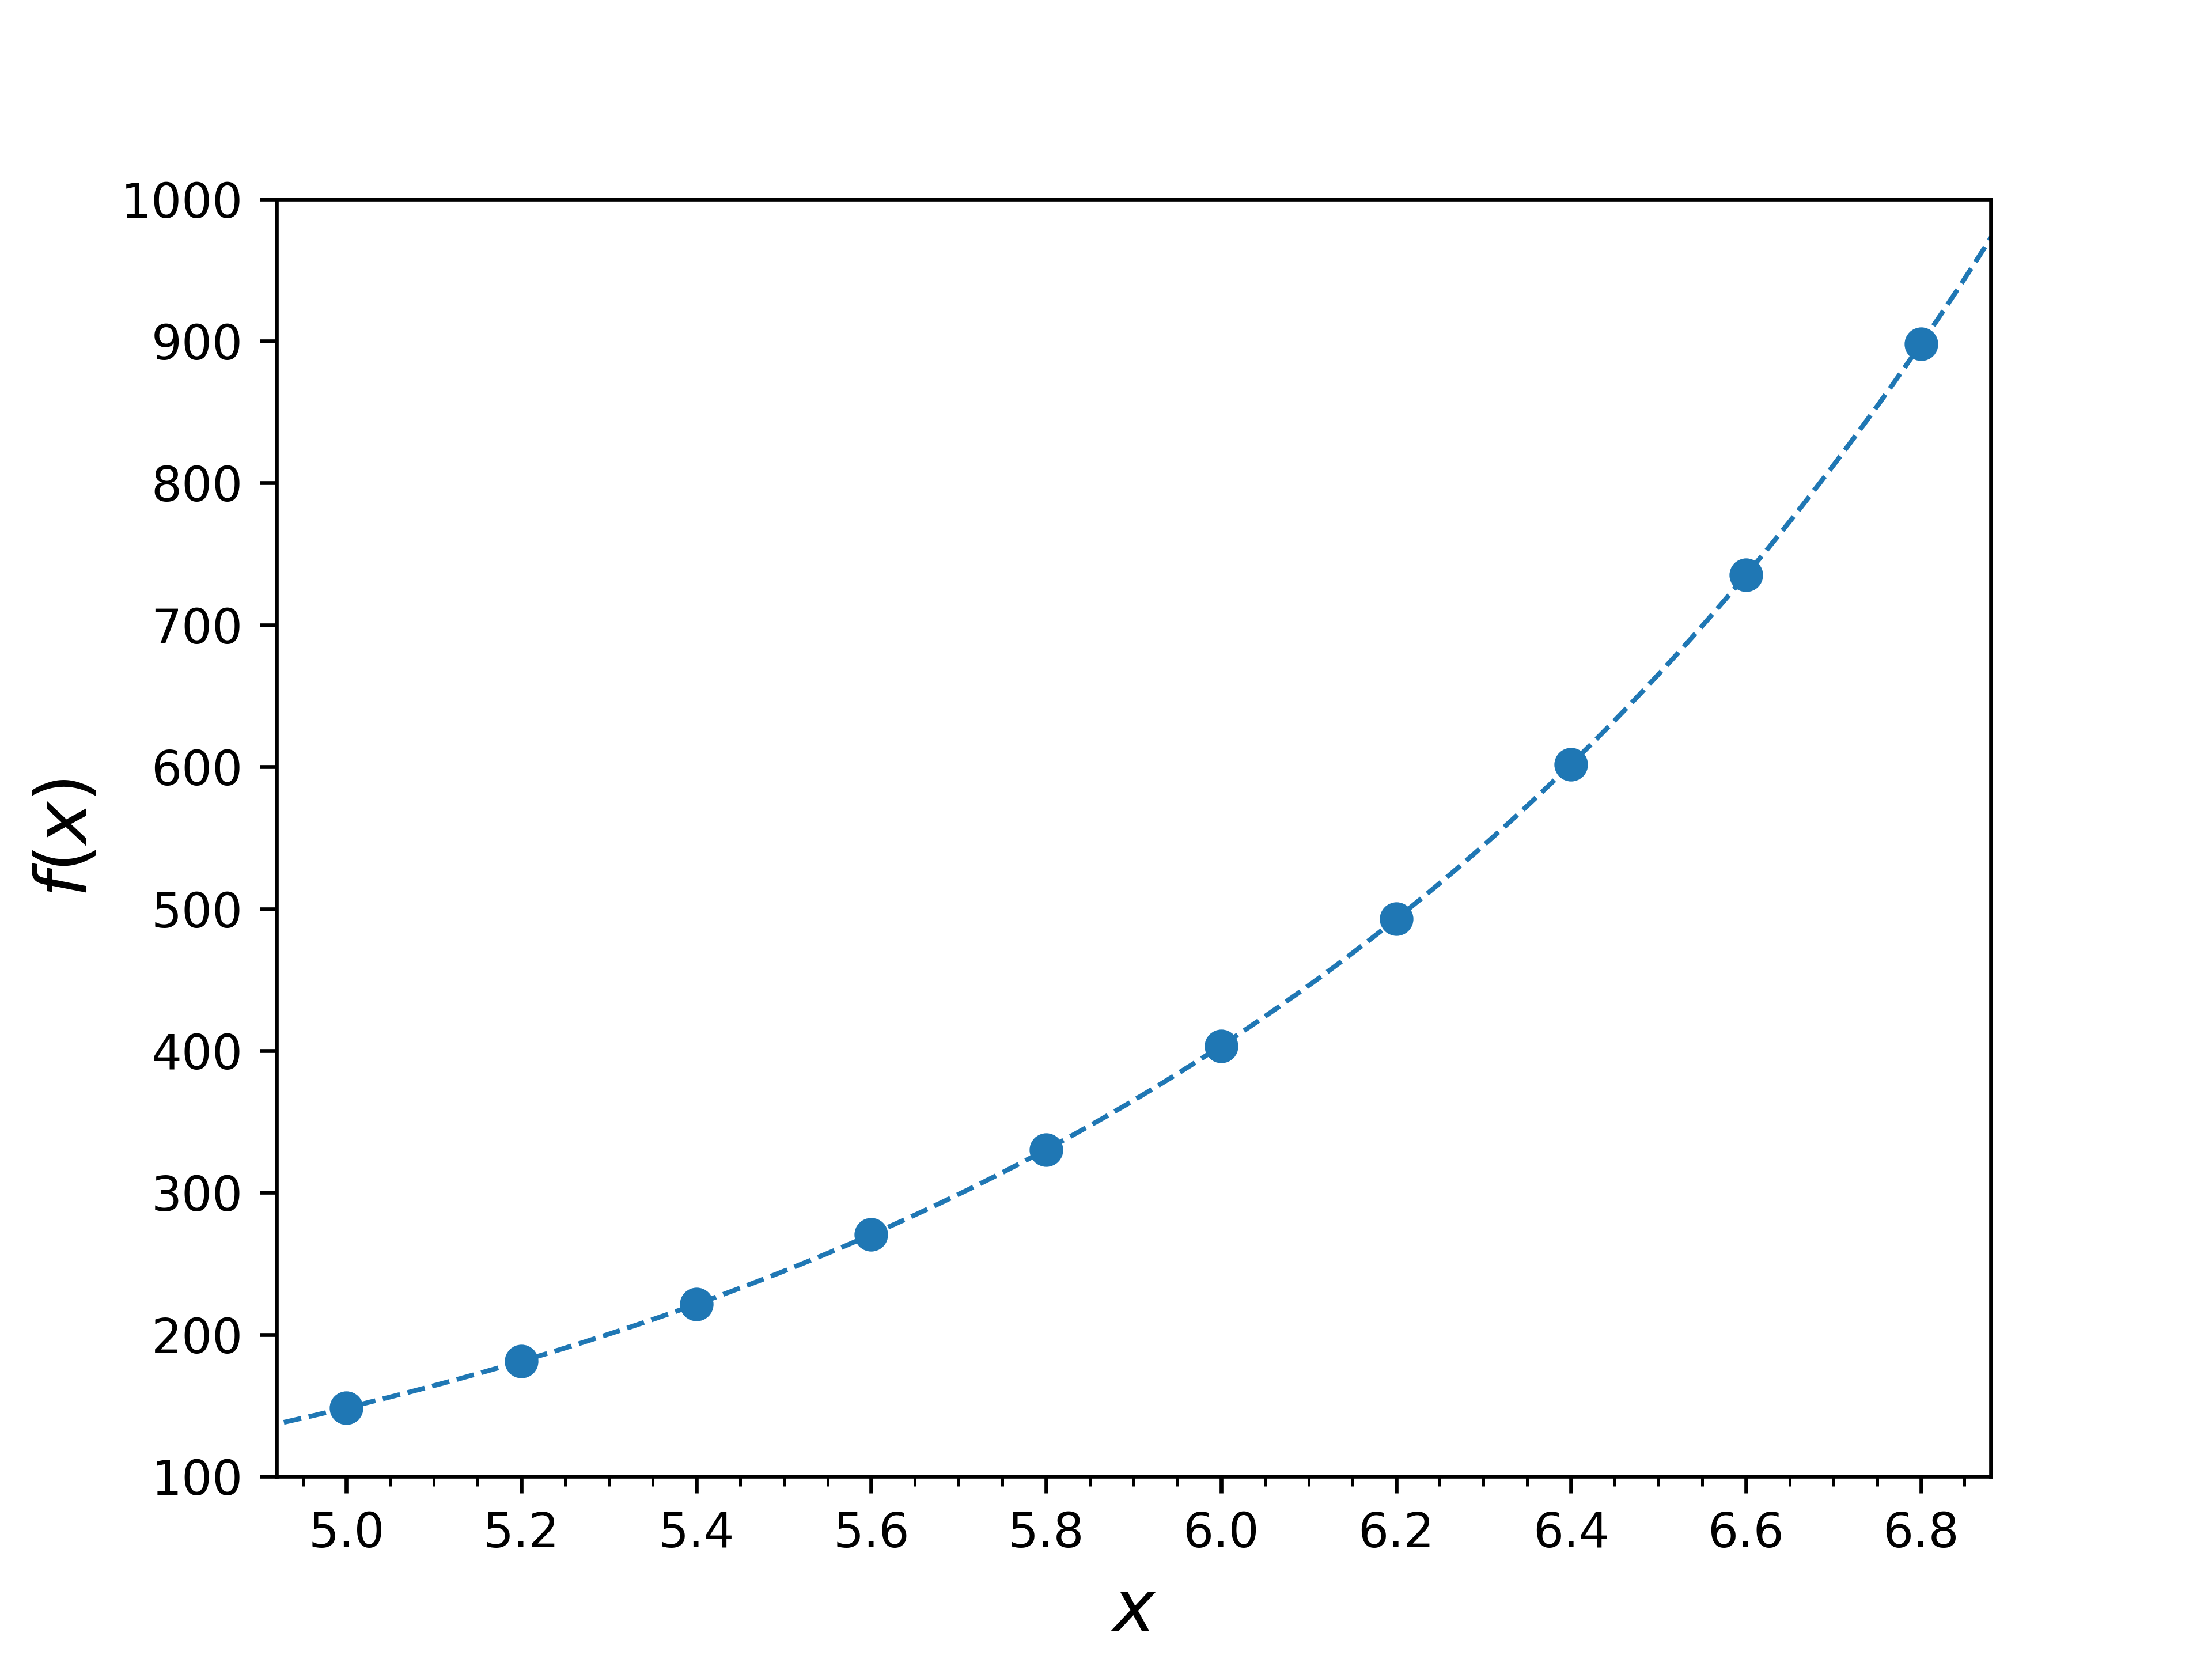
\includegraphics[width=0.75\textwidth]{figures/Fig1.png}
	\caption{Caption.}
	\label{fig:Fig1}
\end{figure*}

I show now the code used to generate this dataset, as well as Figure \ref{fig:Fig1}.

\begin{lstlisting}[language=Python, caption=Code1,backgroundcolor=\color{lightgrey},keywordstyle=\color{darkgreen},commentstyle=\color{red}]
import math
import matplotlib.pyplot as plt 
from matplotlib.ticker import (MultipleLocator)
import random
import numpy as np

### 1) Generate data
list_x = []
list_y = []
random.seed(19)
for i in np.arange(5, 7, 0.2):
    x = i 
    y = math.exp(x)
    list_x.append(x)
    list_y.append(y)
    print("%.2f,%.6f" %(x, y)) 
list_x = np.array(list_x).reshape(-1, 1)
list_y = np.array(list_y)
basic_x = np.arange(4.9, 7.0, 0.01)
basic_y = [math.exp(x) for x in basic_x]
# Plot graph
plt.plot(basic_x,basic_y,color='C0',linestyle='dashed',linewidth=1)
plt.scatter(list_x, list_y,color='C0')
plt.xlabel('$x$',fontsize=15)
plt.ylabel('$f(x)$',fontsize=15)
plt.xticks(np.arange(5,7,0.2))
plt.xlim(4.92,6.88)
plt.ylim(100,1000)
axes = plt.gca()
axes.xaxis.set_minor_locator(MultipleLocator(0.05))
# Save plot into png
file_name='Fig1.png'
plt.savefig(file_name,format='png',dpi=600)
plt.close()
\end{lstlisting}


\section{Cross-validation to optimize k}
test
\section{Uniform vs Distance}
test
\section{Limitations k-NN regression}
test
\end{document}

